\documentclass[problems]{esg8012pset} 
  \usepackage{amsmath}
  \usepackage{amssymb}
  \usepackage{enumerate}
  \usepackage{graphicx}
  \providecommand{\uvec}[1]{{\hat{\bf{#1}}}}
  \usepackage{pgf,tikz}
  \usetikzlibrary{arrows}
\classname{Physics 8.012} 
\semester{Fall 2010} 
\problemsetnumber{2} 
\date{September 17} 
\duedate{Friday, September 24} 
\readingassignment{Kleppner and Kolenkow, \emph {An Introduction to Mechanics}, Chapter Two} 
\begin{document}
\section*{Problem 1: K\&K 2.2}
  The two blocks shown in the figure are connected by a string of negligible mass. If the system is released from rest, find how far the block of mass $m_1$ slides in time $t$. Neglect friction.
  \begin{center}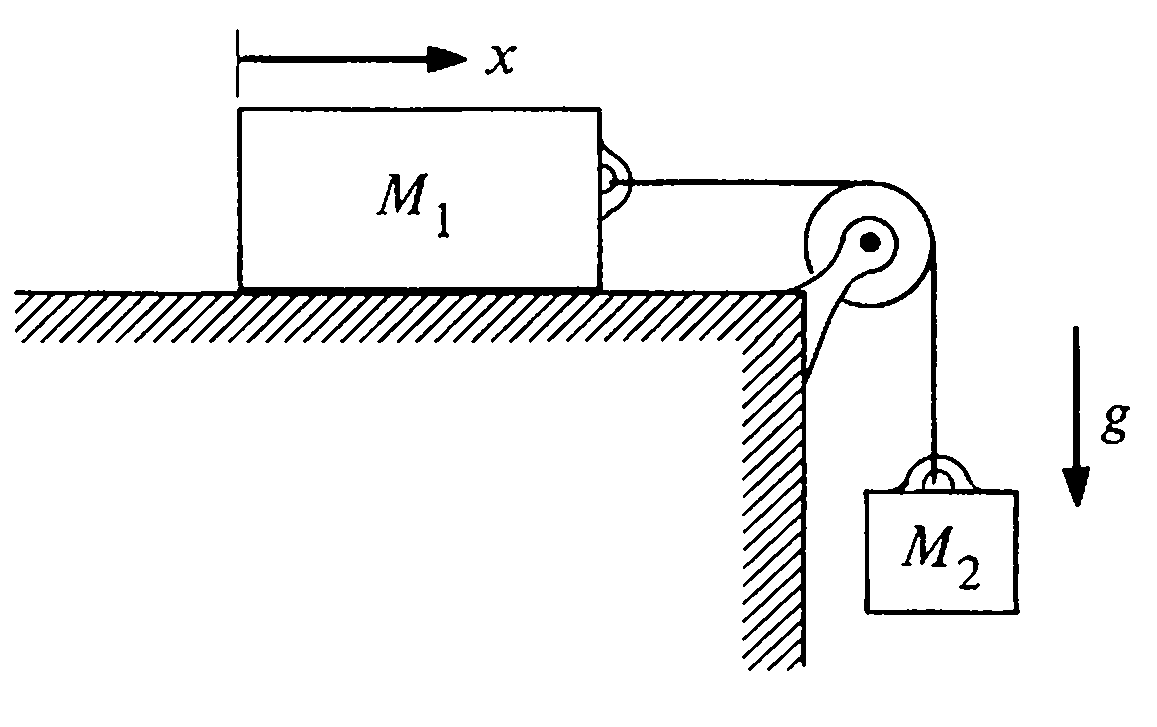
\includegraphics[width=0.35\textwidth]{ps02_1}\end{center}
\section*{Problem 2: K\&K 2.4}
  Two particles of mass $m_1$ and $m_2$ undergo uniform circular motion about each other at a separation $R$ under the influence of an attractive force of magnitude $F$.  The angular velocity is $\omega$ radians per second.
  \begin{enumerate}[a)]
    \item Show that $R = \frac{F}{\omega^2} \cdot \left(\frac{1}{m_1} + \frac{1}{m_2}\right)$.
    \item Explain why you can think of this problem as equivalent to a single body of mass $\mu$ where $\frac{1}{\mu} = \left(\frac{1}{m_1} + \frac{1}{m_2}\right)$ undergoing circular motion of radius $R$ due to the influence of a central attractive force of magnitude $F$.
  \end{enumerate}
\section*{Problem 3: K\&K 2.7}
  Consider two textbooks that are resting one on top of the other. The lower book has $m_2 = 0.8$ kg and is resting on a nearly frictionless surface. The upper book has mass $m_1 = 2.0$ kg. Suppose the coefficient of static friction is given by $\mu_s = 0.1$.
  \begin{center}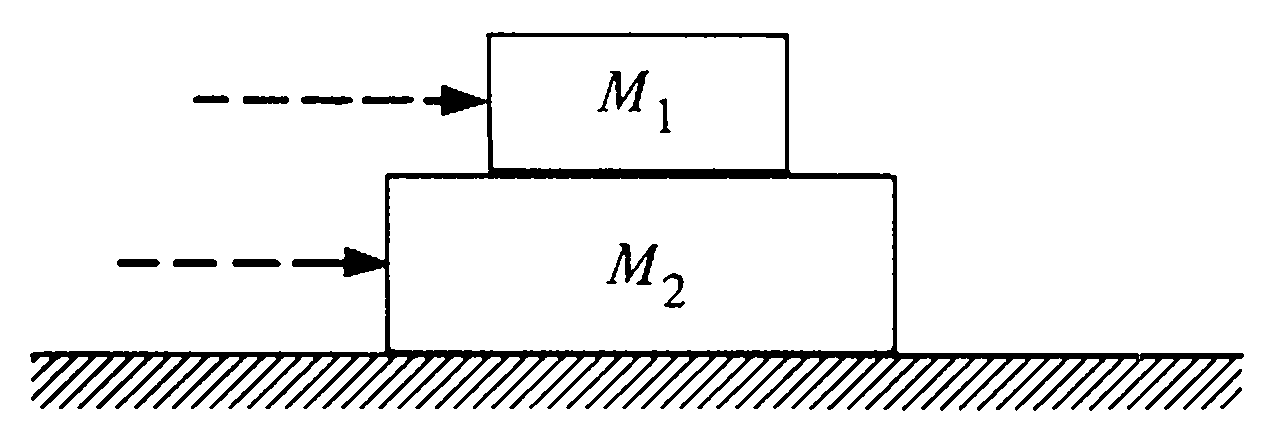
\includegraphics[width=0.35\textwidth]{ps02_2}\end{center}
  \begin{enumerate}[a)]
    \item What is the maximum force which the upper book can be pushed horizontally so that the two books move together without slipping? Identify all action-reaction pairs of forces in this problem.
    \item What is the maximum force which the lower book can be pushed horizontally so that the two books move together without slipping? Identify all action-reaction pairs of forces in this problem.
    \item Explain why one of your forces in parts a) and b) is larger than the other.
  \end{enumerate}
\section*{Problem 4: K\&K 2.9}
  A body of mass $m$ is moving in a horizontal circle of radius $r$ with a constant speed $v_0$ on the inside wall of a cone. Assume the wall of the cone is frictionless. The wall of the cone makes an angle $\theta$ with the vertical.
  \begin{center}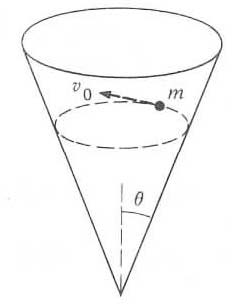
\includegraphics[width=0.2\textwidth]{ps02_3}\end{center}
  \begin{enumerate}[a)]
    \item Draw a free body force diagram showing all the forces acting on the mass.
    \item What is the speed, $v_0$, of the body, in terms of $r$, $m$, $\theta$, and $g$?
    \item How long will the mass take to go around the circle?
    \item Now assume there is a coefficient of static friction $\mu_s$. Find the maximum speed the mass can move on the inside of a cone and still move in a circular orbit of radius $r$.
  \end{enumerate}
\section*{Problem 5: K\&K 2.10}
  The earth is spinning about its axis with a period of 23 hours 56 min and 4 sec. The equatorial radius of the earth is $6.38\cdot 10^{6}$ m. The latitude of Cambridge, Mass is 42$^{\circ}$ 22'.
  \begin{enumerate}[a)]
    \item Find the velocity of a person at MIT as they undergo circular motion about the earth? axis of rotation.
    \item Find the person's centripetal acceleration.
    \item The rotation of the Earth is slowing down. In 1977, the Earth took 1.01s longer to complete 365 rotations than in 1900. What was the average angular deceleration of the Earth in the time interval from 1900 to 1977?
    \item Find the radius of the orbit of a synchronous satellite which circles the earth. (A synchronous satellite goes around the earth once every rotation of the earth, so that its position appears stationary with respect to a ground station).  \par\noindent
      Note: You may need to use the fact that the force of gravity between two objects of masses $m_1$ and $m_2$, separated by a distance $d$, is $F_g = \frac{G m_1 m_2}{d^2}$, where $G$ is the universal constant of gravitation.
  \end{enumerate}
\section*{Problem 6: K\&K 2.16}
  A 45$^{\circ}$ wedge is pushed along a table with constant acceleration $A$. A block of mass $m$ slides without friction down the wedge. Find its acceleration. (Gravity is directed down.)
  \begin{center}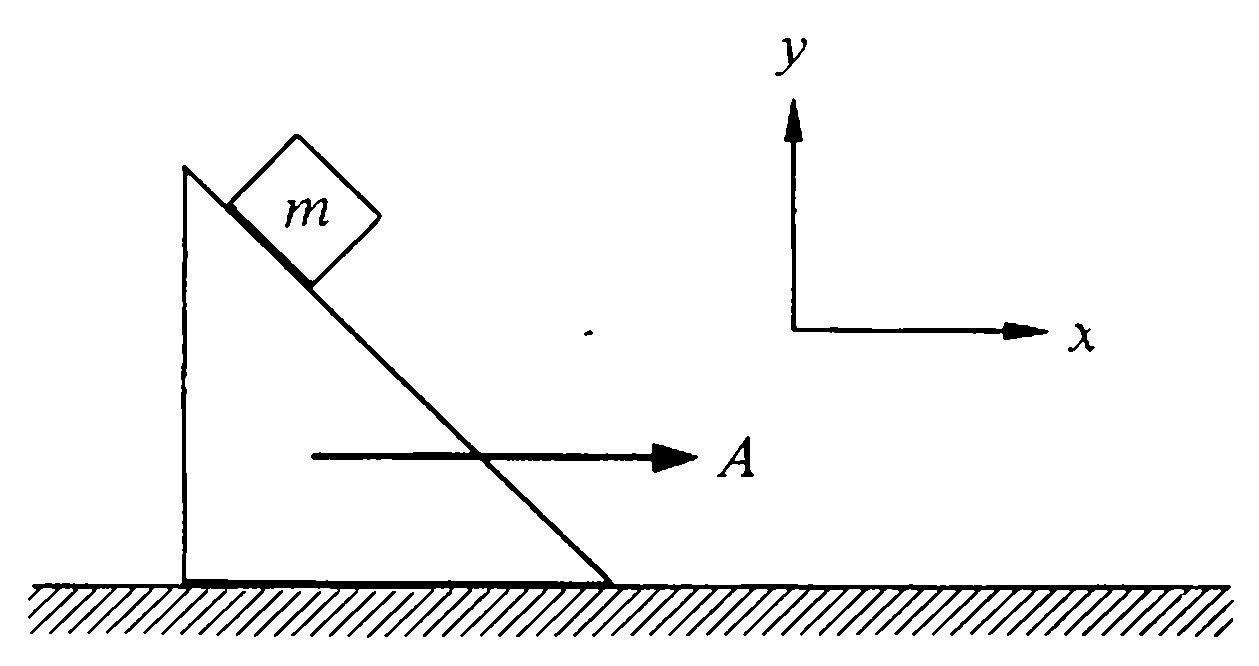
\includegraphics[width=0.35\textwidth]{ps02_4}\end{center}
\section*{Problem 7: K\&K 2.22}
  Suppose a rope of mass $m$ hangs between two trees. The ends of the rope are at the same height and they make an angle $\theta$ with the trees.
  \begin{center}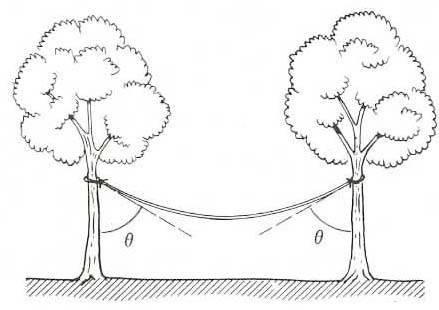
\includegraphics[width=0.35\textwidth]{ps02_5}\end{center}
  \begin{enumerate}[a)]
    \item What is the tension at the ends of the rope where it is connected to the trees?
    \item What is the tension in the rope at a point midway between the trees?
  \end{enumerate}
\end{document}
